%***************************************************************************************
\section{Prior Uncertainty Propagation of the FEBA Tests}\label{app:tbl_results_uq_feba}
%***************************************************************************************

%--------------------------------------------------------------------------
\subsection{Clad Temperature Output (TC)}\label{app:tbl_results_uq_feba_tc}
%--------------------------------------------------------------------------

% FEBA Test No. 214 Prior Uncertainty Propagation, TC
\rotatebox{90}{\begin{minipage}{0.85\textheight}
    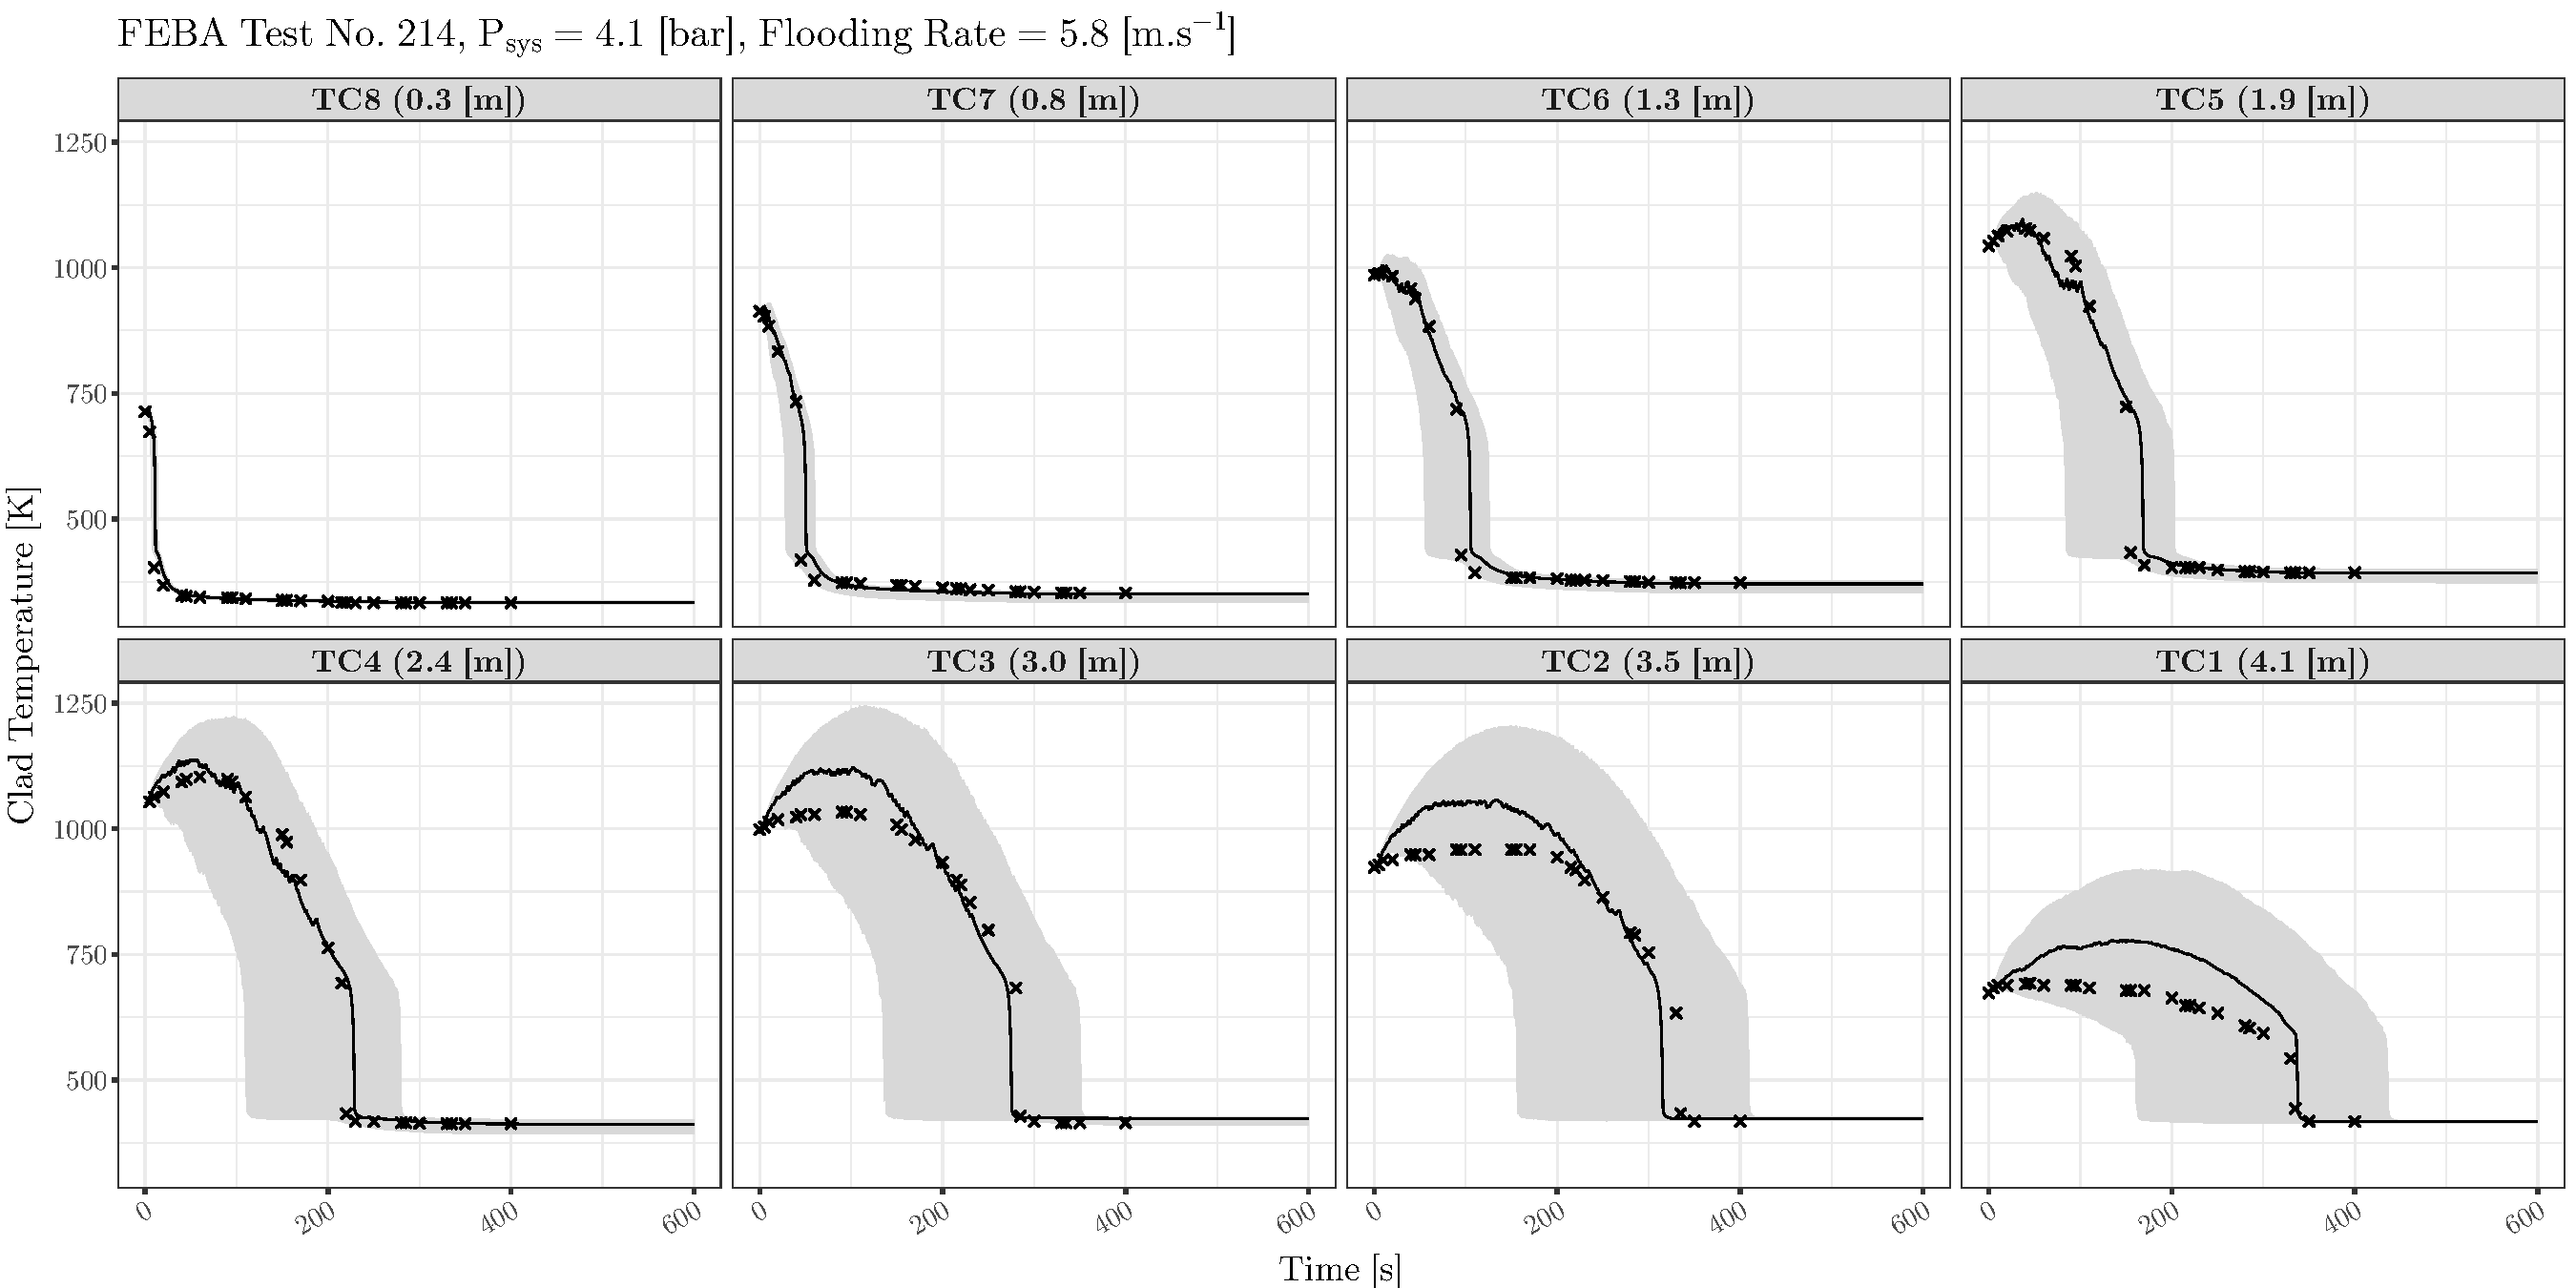
\includegraphics[width=1\textwidth]{../figures/chapter2/figures/plotTraceUQPriorTC214}
		\captionof{figure}[Prior uncertainty propagation of FEBA Test No. $214$ for the cladding temperature output ($TC$).]{Uncertainty propagation of the prior parameters uncertainty of \gls[hyper=false]{feba} Test No. $214$ for the cladding temperature output ($TC$) at different axial locations using \gls[hyper=false]{trace}. The uncertainty bound refers to the symmetric ($95\%$) probability, solid lines indicate the simulation with the nominal parameters values, and crosses indicate the experimental data.}
    \label{fig:ch2_plot_trace_uq_prior_tc_214}
\end{minipage}}

% FEBA Test No. 218 Prior Uncertainty Propagation, TC
\clearpage
\begin{sidewaysfigure}
	\centering
	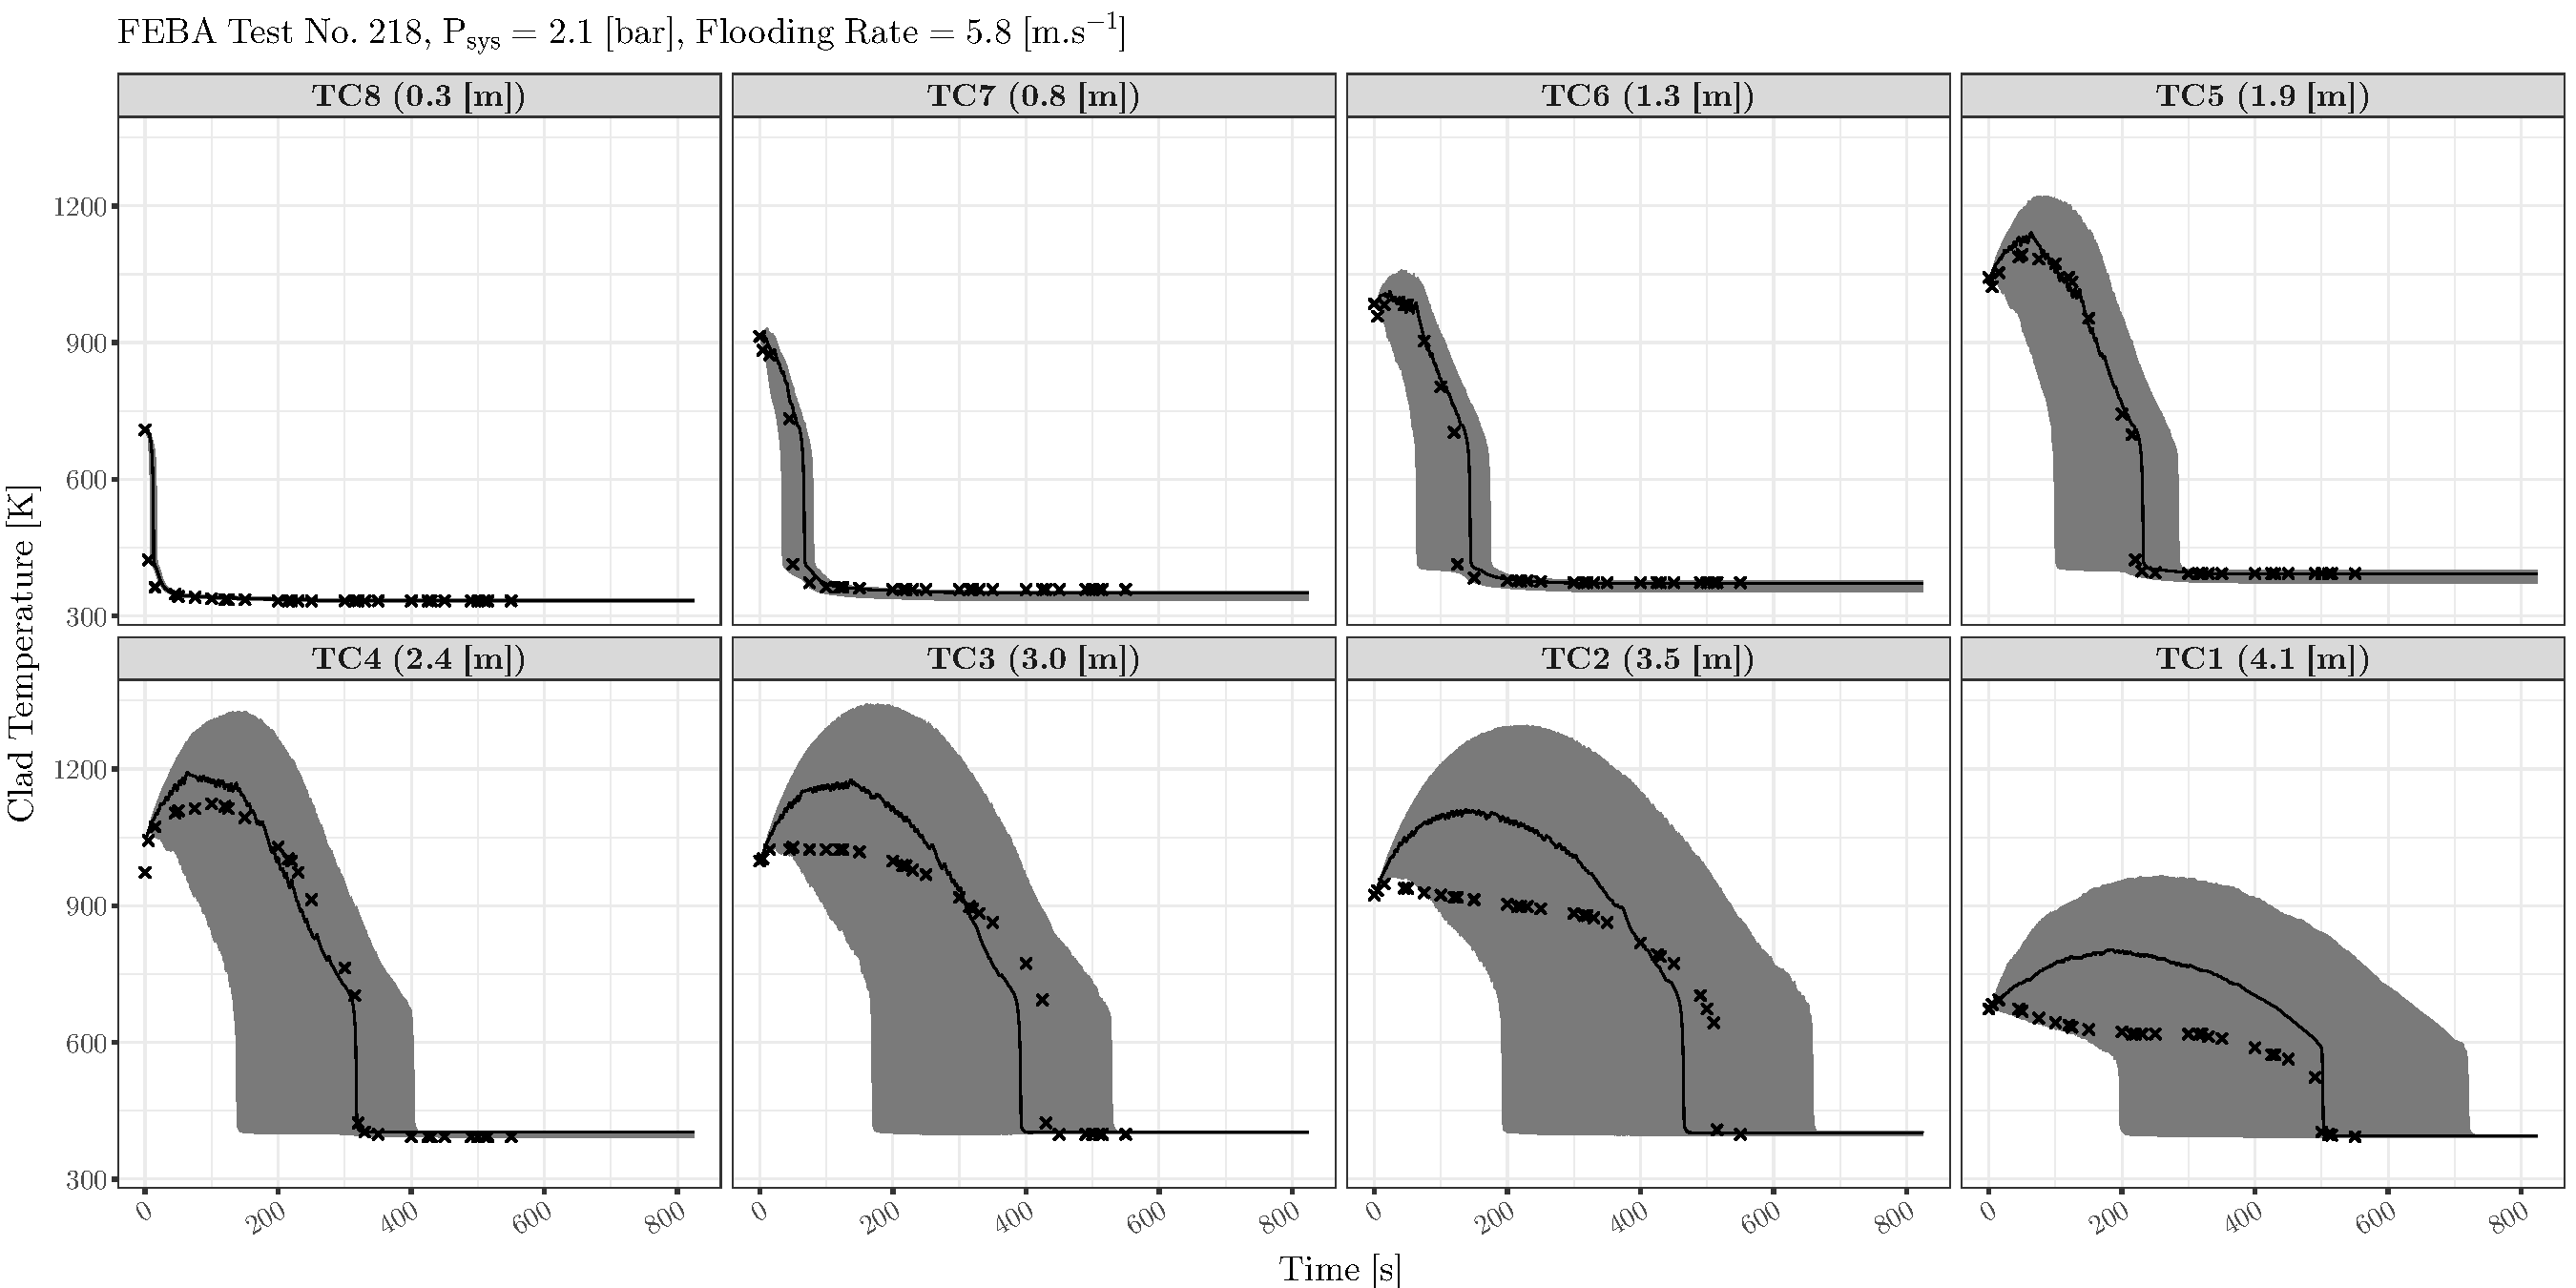
\includegraphics[width=1.0\textwidth]{../figures/chapter2/figures/plotTraceUQPriorTC218}
		\captionof{figure}[Prior uncertainty propagation of FEBA Test No. $218$ for the cladding temperature output ($TC$).]{Uncertainty propagation of the prior parameters uncertainty of \gls[hyper=false]{feba} Test No. $218$ for the cladding temperature output ($TC$) at different axial locations using \gls[hyper=false]{trace}. The uncertainty bound refers to the symmetric ($95\%$) probability, solid lines indicate the simulation with the nominal parameters values, and crosses indicate the experimental data.}
	\label{fig:ch2_plot_trace_uq_prior_tc_218}
\end{sidewaysfigure}
\clearpage

% FEBA Test No. 223 Prior Uncertainty Propagation, TC
\clearpage
\begin{sidewaysfigure}
	\centering
	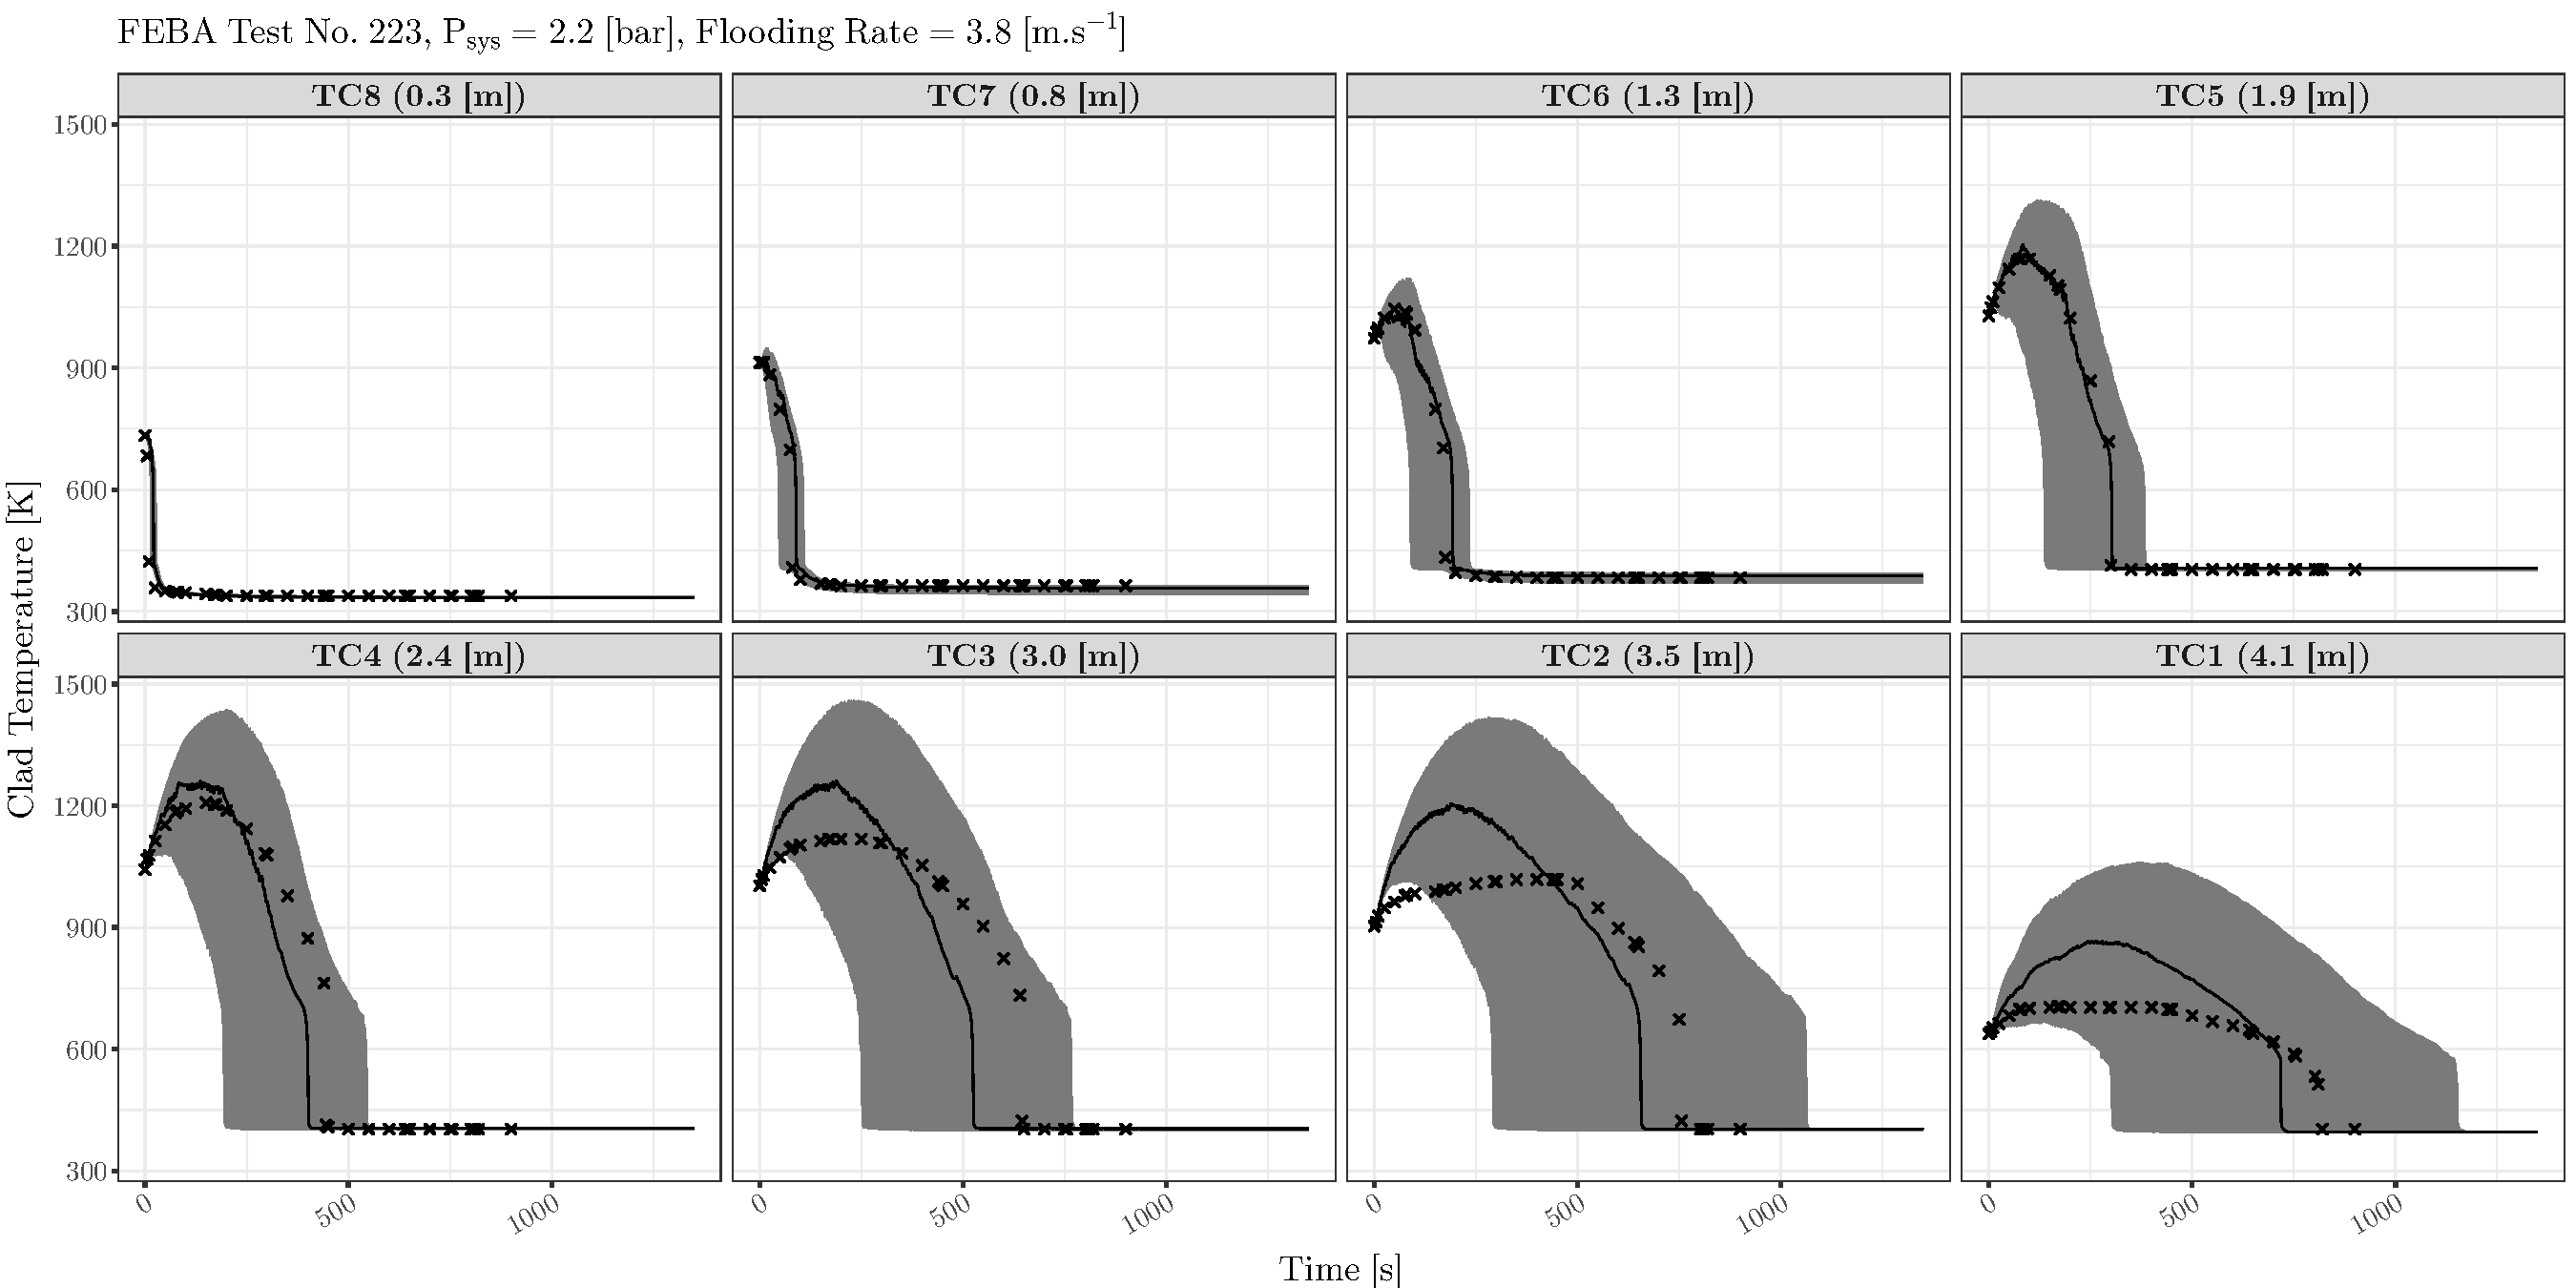
\includegraphics[width=1.0\textwidth]{../figures/chapter2/figures/plotTraceUQPriorTC223}
		\captionof{figure}[Prior uncertainty propagation of FEBA Test No. $223$ for the cladding temperature output ($TC$).]{Uncertainty propagation of the prior parameters uncertainty of \gls[hyper=false]{feba} Test No. $223$ for the cladding temperature output ($TC$) at different axial locations using \gls[hyper=false]{trace}. The uncertainty bound refers to the symmetric ($95\%$) probability, solid lines indicate the simulation with the nominal parameters values, and crosses indicate the experimental data.}
	\label{fig:ch2_plot_trace_uq_prior_tc_223}
\end{sidewaysfigure}
\clearpage

% FEBA Test No. 220 Prior Uncertainty Propagation, TC
\clearpage
\begin{sidewaysfigure}
	\centering
	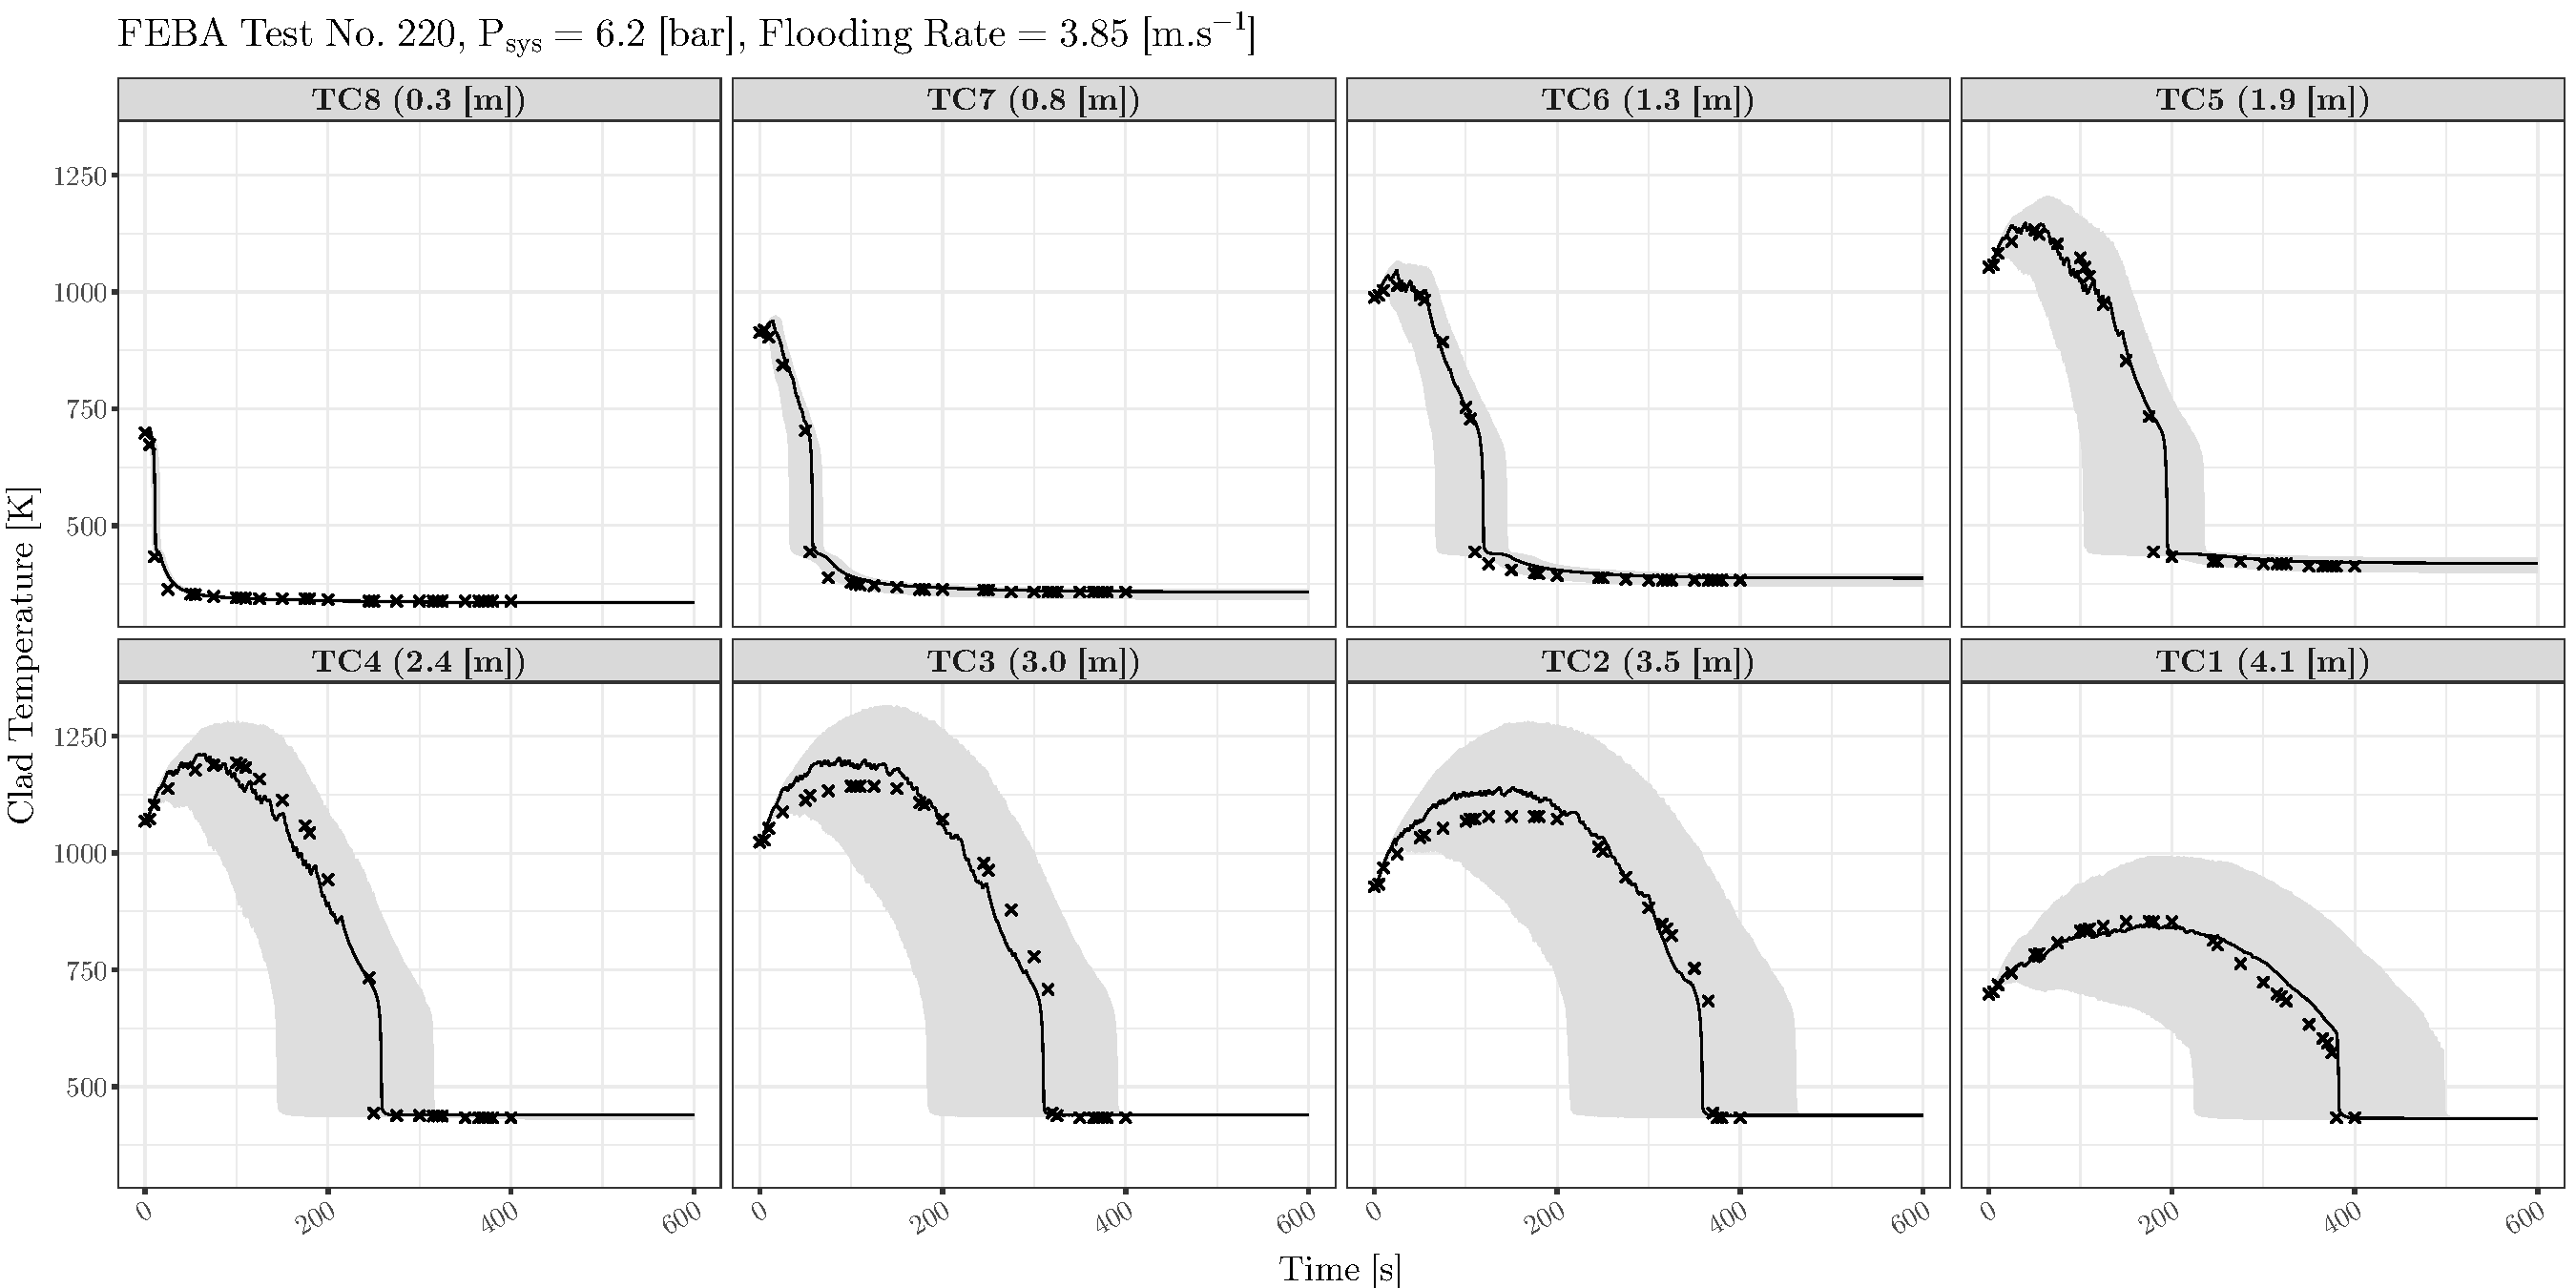
\includegraphics[width=1.0\textwidth]{../figures/chapter2/figures/plotTraceUQPriorTC220}
		\captionof{figure}[Prior uncertainty propagation of FEBA Test No. $220$ for the cladding temperature output ($TC$).]{Uncertainty propagation of the prior parameters uncertainty of \gls[hyper=false]{feba} Test No. $220$ for the cladding temperature output ($TC$) at different axial locations using \gls[hyper=false]{trace}. The uncertainty bound refers to the symmetric ($95\%$) probability, solid lines indicate the simulation with the nominal parameters values, and crosses indicate the experimental data.}
	\label{fig:ch2_plot_trace_uq_prior_tc_223}
\end{sidewaysfigure}
\clearpage

% FEBA Test No. 222 Prior Uncertainty Propagation, TC
\clearpage
\begin{sidewaysfigure}
	\centering
	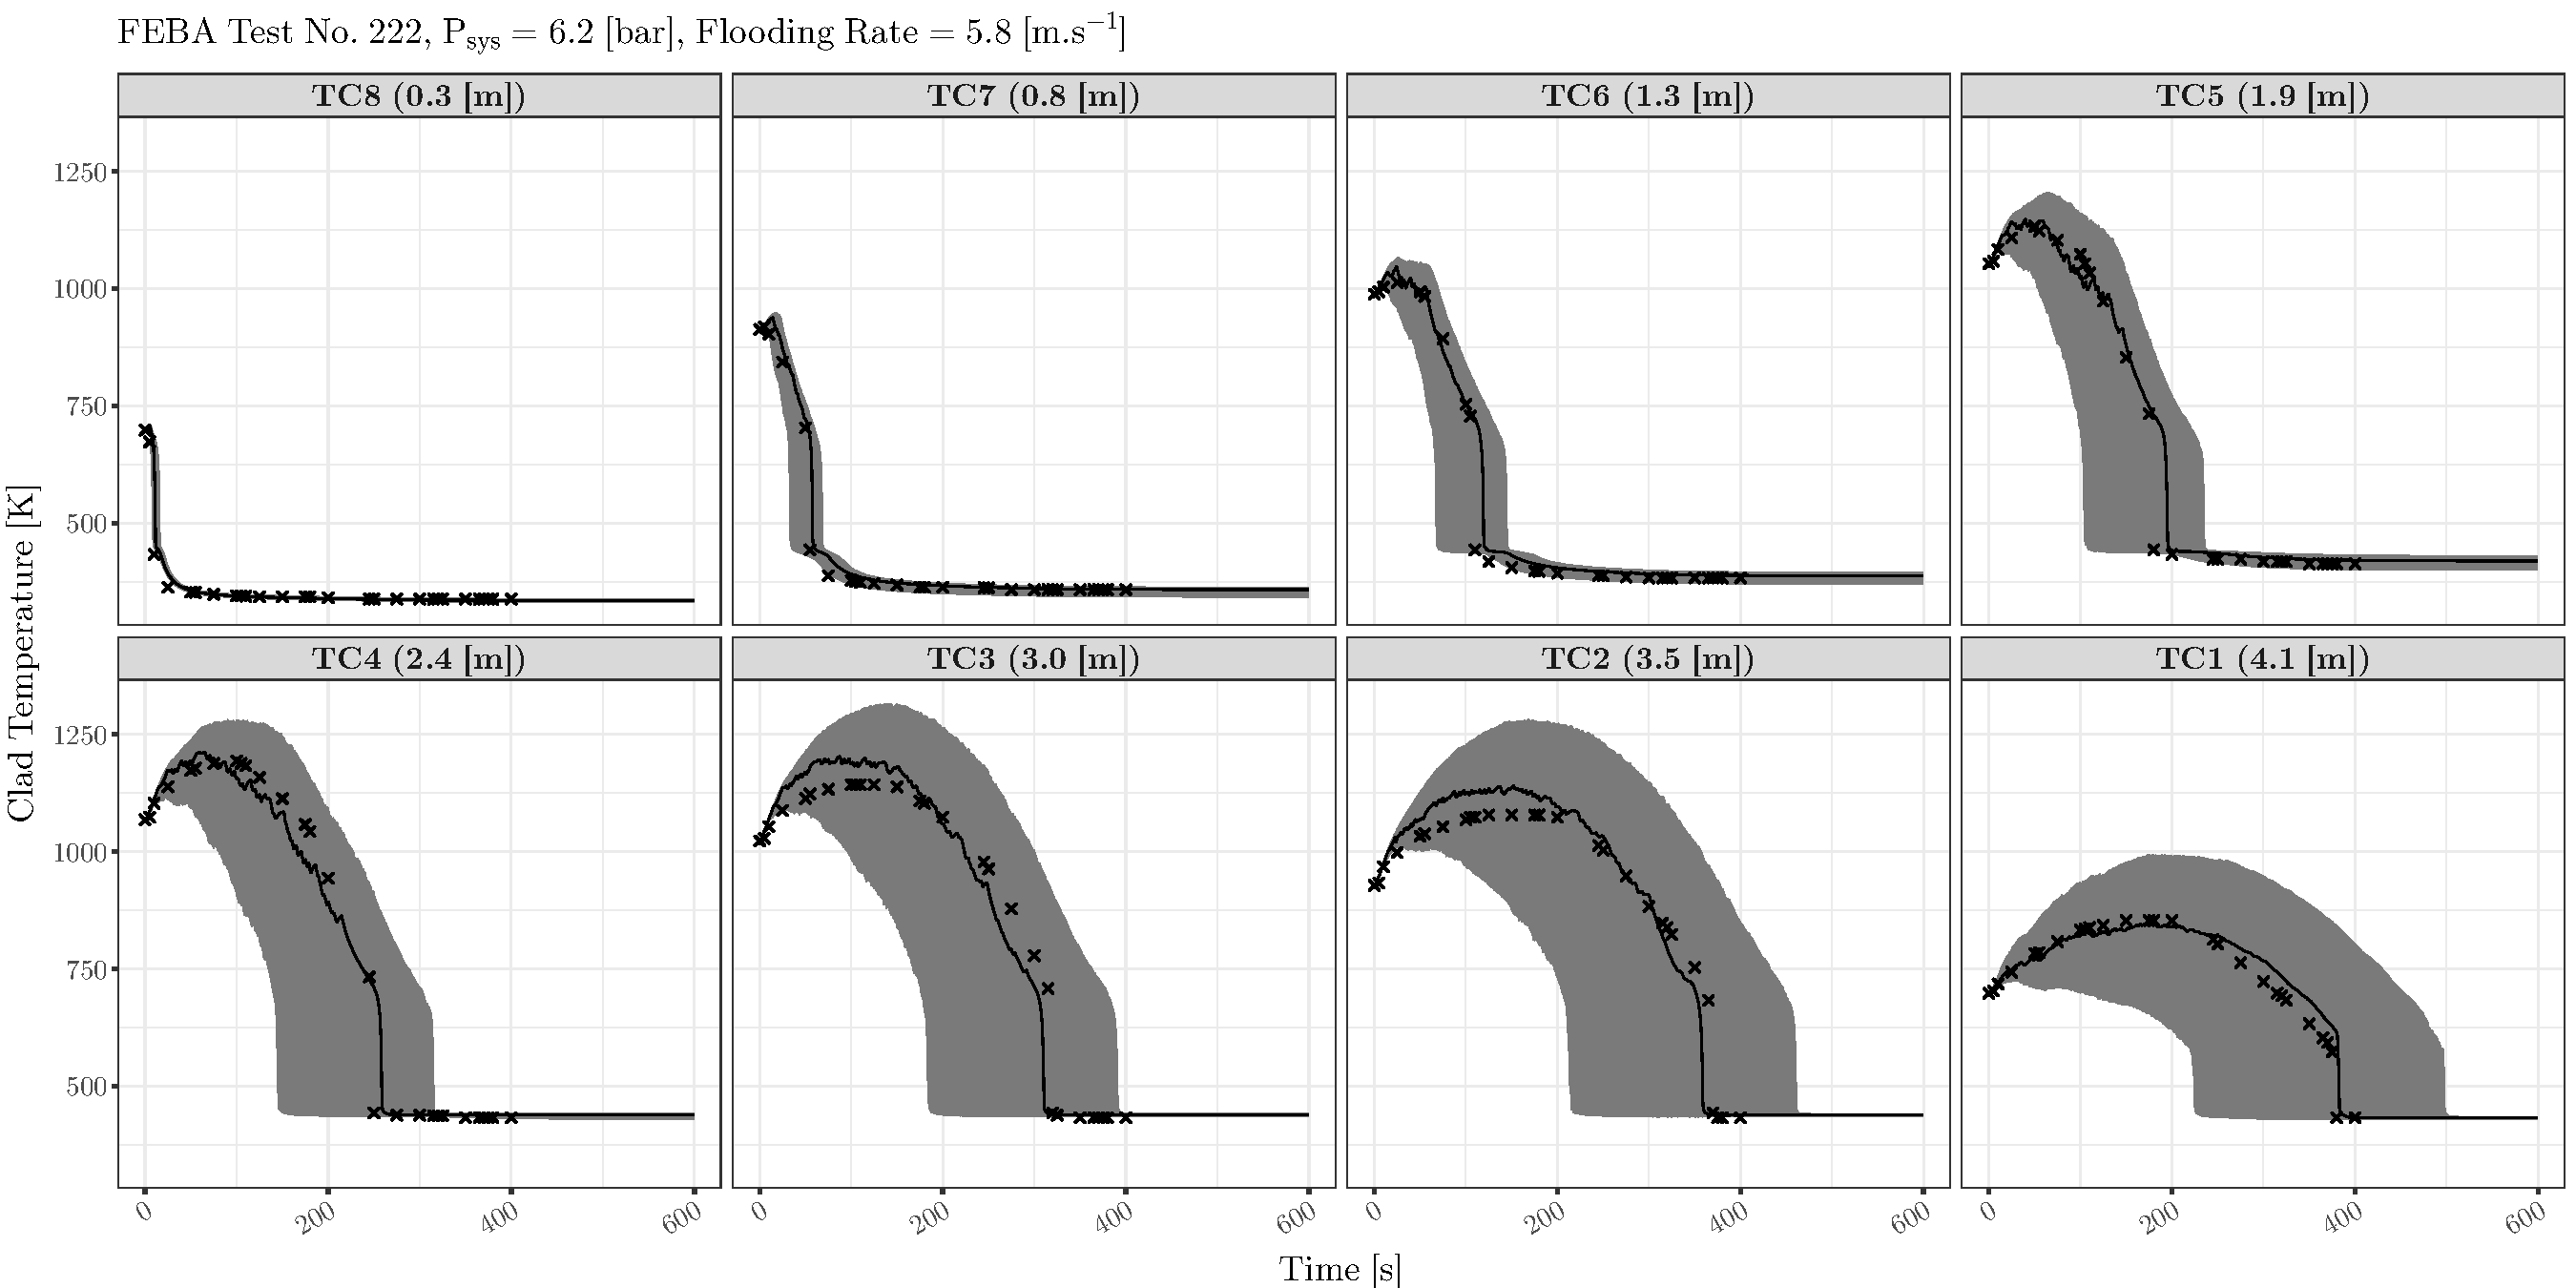
\includegraphics[width=1.0\textwidth]{../figures/chapter2/figures/plotTraceUQPriorTC222}
		\captionof{figure}[Prior uncertainty propagation of FEBA Test No. $222$ for the cladding temperature output ($TC$).]{Uncertainty propagation of the prior parameters uncertainty of \gls[hyper=false]{feba} Test No. $222$ for the cladding temperature output ($TC$) at different axial locations using \gls[hyper=false]{trace}. The uncertainty bound refers to the symmetric ($95\%$) probability, solid lines indicate the simulation with the nominal parameters values, and crosses indicate the experimental data.}
	\label{fig:ch2_plot_trace_uq_prior_tc_223}
\end{sidewaysfigure}
\clearpage

%-----------------------------------------------------------------------
\subsection{Pressure Drop Output (DP)}\label{app:tbl_results_uq_feba_dp}
%-----------------------------------------------------------------------

% FEBA Test No. 214 Prior Uncertainty Propagation, DP
\begin{figure}[bth]
    \centering
    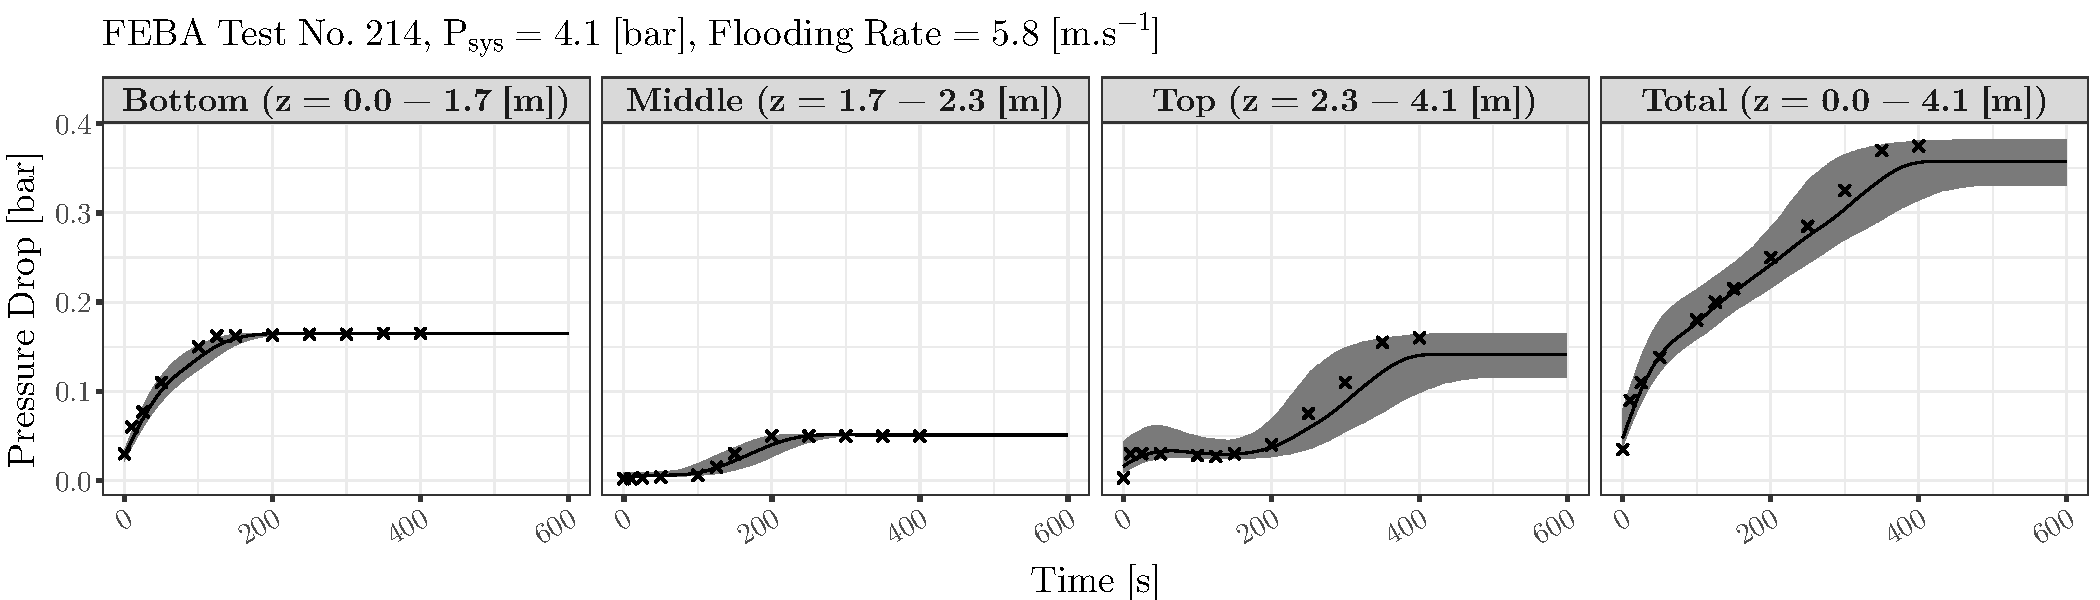
\includegraphics[width=1.0\textwidth]{../figures/chapter2/figures/plotTraceUQPriorDP214}
    \caption[Prior uncertainty propagation of FEBA Test No. $214$ for the pressure drop output ($DP$).]{Uncertainty propagation of the prior parameters uncertainty of \gls[hyper=false]{feba} Test No. $214$ for the pressure drop output ($TC$) at different axial segments using \gls[hyper=false]{trace}. The uncertainty bound refers to the symmetric ($95\%$) probability, solid lines indicate the simulation with the nominal parameters values, and crosses indicate the experimental data.}
    \label{fig:ch2_plot_trace_uq_prior_dp_214}
\end{figure}

% FEBA Test No. 218 Prior Uncertainty Propagation, DP
\begin{figure}[bth]
    \centering
    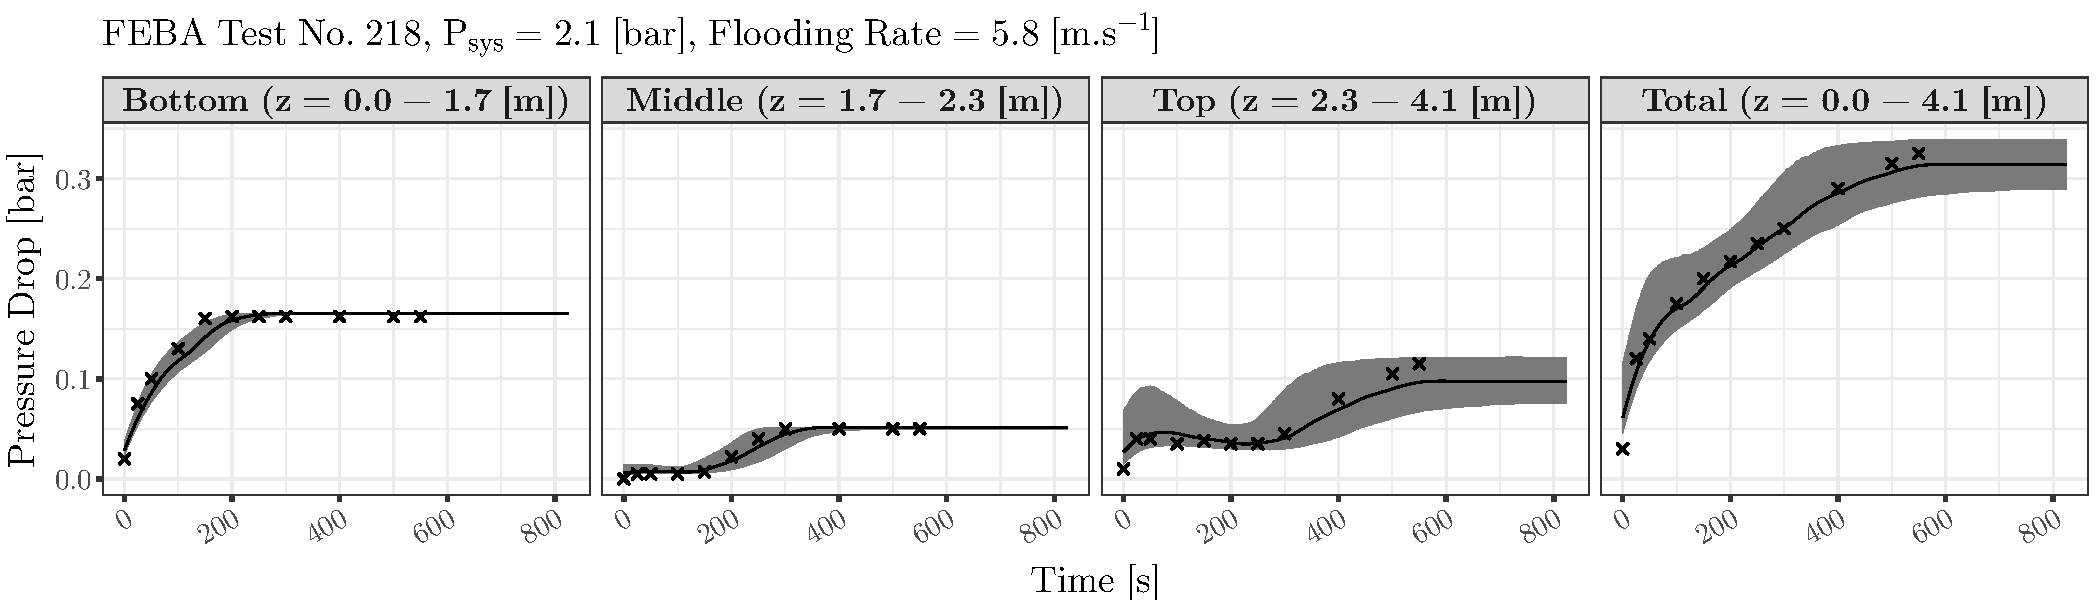
\includegraphics[width=1.0\textwidth]{../figures/chapter2/figures/plotTraceUQPriorDP218}
    \caption[Prior uncertainty propagation of FEBA Test No. $218$ for the pressure drop output ($DP$).]{Uncertainty propagation of the prior parameters uncertainty of \gls[hyper=false]{feba} Test No. $218$ for the pressure drop output ($TC$) at different axial segments using \gls[hyper=false]{trace}. The uncertainty bound refers to the symmetric ($95\%$) probability, solid lines indicate the simulation with the nominal parameters values, and crosses indicate the experimental data.}
    \label{fig:ch2_plot_trace_uq_prior_dp_218}
\end{figure}

%--------------------------------------------------------------------------
\subsection{Liquid carryover Output (CO)}\label{app:tbl_results_uq_feba_co}
%--------------------------------------------------------------------------

\normdoublefigure[pos=tbhp,
                  mainlabel={fig:ch2_plot_trace_uq_prior_co_1},
                  maincaption={},
				mainshortcaption={Prior uncertainty propagation of FEBA Test No. $214$-$218$ for the liquid carryover output ($CO$).},
                  leftopt={width=0.45\textwidth},
                  leftlabel={fig:ch2_plot_trace_uq_prior_co_214},
                  leftcaption={\gls[hyper=false]{feba} Test No. 214},
                  %leftshortcaption={},%
                  rightopt={width=0.45\textwidth},
                  rightlabel={fig:ch2_plot_trace_uq_prior_co_218},
                  rightcaption={\gls[hyper=false]{feba} Test No. 218}]
{../figures/chapter2/figures/plotTraceUQPriorCO214.pdf}
{../figures/chapter2/figures/plotTRACEUQPriorCO218.pdf}